\documentclass[12pt]{article}
\usepackage[a4paper]{geometry}
\usepackage{fullpage}
\usepackage[T1]{fontenc}
\usepackage[utf8]{inputenc}
\usepackage{graphicx}
\usepackage{mathpazo}
\pagenumbering{gobble}
\usepackage{siunitx}
\DeclareSIUnit\voltampere{VA}
\DeclareSIUnit\kWh{kWh}
\usepackage{amsmath}
\usepackage[spanish]{babel}
\usepackage{steinmetz}

\renewcommand{\thesection}{Problema \arabic{section}}

\begin{document}

\title{}

\date{Curso 2020-21}

\section{}

Un generador cuya fuerza electromotriz es de \SI{120}{V} y resistencia interna \SI{0.2}{\ohm}, entrega una corriente de \SI{20}{\ampere} a un motor situado a \SI{300}{\meter} de distancia y de resistencia interna \SI{0.5}{\ohm}. La línea es de cobre de resistividad $\SI{17.24}{\milli\ohm\milli\meter\squared\per\meter}$. Sabiendo que el motor absorbe \SI{10.2}{\kWh} en 5 horas, hallar: 
\begin{enumerate}
\item Fuerza contraelectromotriz del motor.
\item Sección de los conductores.
\item Rendimiento del motor, del generador, de la línea y rendimiento total.
\item Balance general de potencias.
\end{enumerate}

\section{}
Un generador de corriente continua alimenta a dos cargas. La primera está situada a \SI{2100}{\meter}, tiene una resistencia de \SI{215}{\ohm} y rendimiento unidad. La segunda está situada a \SI{270}{\meter} después de la primera, tiene una potencia de \SI{4662}{\watt}, un rendimiento del 75\%, y una tensión aplicada de \SI{420}{\volt}.

Sabiendo que la línea es de cobre, de \SI{6}{\milli\meter\squared} de sección, y que la resistividad es de $\SI{17.24}{\milli\ohm\milli\meter\squared\per\meter}$, determinar:

\begin{enumerate}
\item Tensión en bornes del generador.
\item Intensidad entregada por el generador.
\item Rendimiento de la instalación.
\end{enumerate}

\section{}

Convierte en fuente de tensión o intensidad, según corresponda.

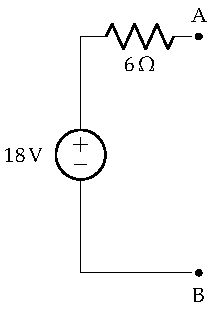
\includegraphics{figs/Conversion_Fuentes.pdf}
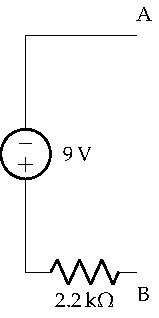
\includegraphics{figs/Conversion_Fuentes_2.pdf}
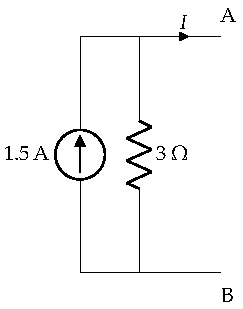
\includegraphics{figs/Conversion_Fuentes_3.pdf}
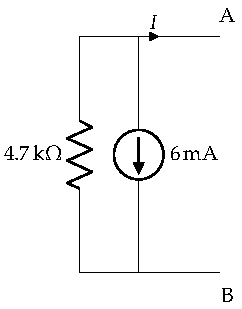
\includegraphics{figs/Conversion_Fuentes_4.pdf}

\section{}

Calcula la resistencia equivalente entre A y B.

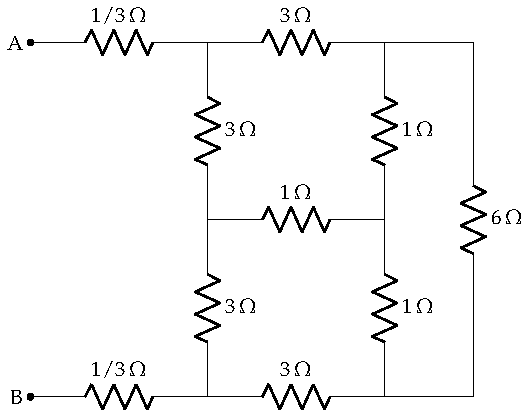
\includegraphics{figs/CircuitoResistivo_FM.pdf}

\section{}

Analiza el circuito de la figura mediante el método de las mallas, obteniendo:
\begin{enumerate}
\item Corriente de cada una de las ramas
\item Potencial en cada uno de los nudos, tomando como referencia el
  nudo A.
\end{enumerate}

Con estos resultados, realiza un balance de potencias comparando la potencia de los elementos activos y la de los elementos pasivos.

\begin{minipage}{0.4\linewidth}
  Datos:
  \begin{align*}
    R_1 = R_3 = R_6 &= \SI{3}{\ohm}\\
    R_2 = R_4 = R_5 &= \SI{2}{\ohm}\\
    \epsilon_1 &= \SI{245}{\volt}\\
    \epsilon_2 &= \SI{490}{\volt}\\
    \epsilon_3 &= \SI{735}{\volt}\\
  \end{align*}
\end{minipage}
\begin{minipage}{0.6\linewidth}
  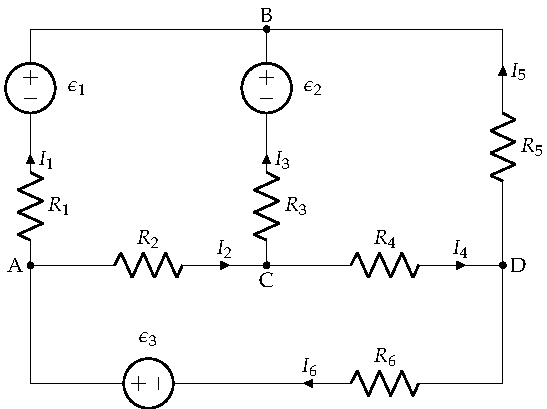
\includegraphics{figs/mallas1.pdf}
\end{minipage}

\section{}
Analiza el circuito de la figura mediante el método de las mallas, obteniendo la corriente de cada una de las ramas. Con este resultado calcula la diferencia de potencial entre A y B, y realiza un balance de potencias comparando la potencia de los elementos activos y la de los elementos pasivos.

\begin{minipage}{0.4\linewidth}
  Datos:
  \begin{align*}
    R_1 = R_2 &= \SI{1}{\ohm}\\
    R_3 &= \SI{2}{\ohm}\\
    R_4 &= \SI{3}{\ohm}\\
    R_5 &= \SI{4}{\ohm}\\
    \epsilon_1 &= \SI{118}{\volt}\\
    \epsilon_2 &= \SI{236}{\volt}\\
    \epsilon_3 &= \SI{118}{\volt}\\
  \end{align*}
\end{minipage}
\begin{minipage}{0.6\linewidth}
  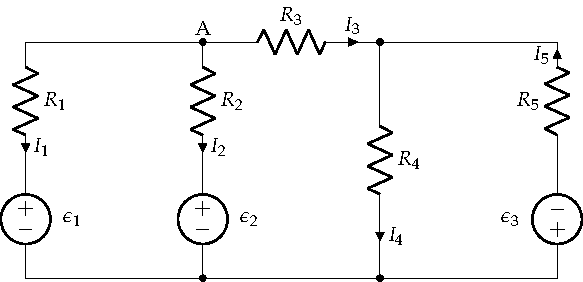
\includegraphics{figs/mallas2.pdf}
\end{minipage}

\end{document}





